\documentclass[11pt]{article}
%基于北京航空航天大学仪器科学与光电工程学院实验报告及课程报告排版得来,类似于毕业论文排版格式
%后续将更新毕业论文排版格式
\usepackage{graphicx,float}%使用图的宏包,使用图的浮动体宏包,引入参数H使图像紧跟当前文字
\usepackage{caption} %使用图表标题的宏包
\usepackage[colorlinks=true,pdfstartview=FitH,%
linkcolor=black,anchorcolor=violet,citecolor=magenta]{hyperref}%加载hyperref宏包,使用超链接
\usepackage{setspace}%用于设置行间距列间距等命令的宏包
\usepackage{array}%设置列表高度宽度的宏包
\usepackage{zhnumber}%使用中文数字编号的宏包
\usepackage{titlesec,titletoc}%使用标题自定义形式的宏包和使用目录自定义形式的宏包
\usepackage{siunitx}%物理学单位宏包
\usepackage{tabularx}%让表格宽度等于页面宽度
\usepackage{makecell}%单个表格单元调整的宏包
\usepackage{subfigure} %%使用子图的宏包
\usepackage[backend=biber,%后端backend使用biber
gbnamefmt=lowercase,%将文献作者姓氏区分大小写
bibstyle=gb7714-2015,%加载参考文献样式表
%nature,%%加载biblatex宏包,使用参考文献
citestyle=gb7714-2015,%加载引注样式
%backref=false,%不显示引用文献的页码
gblocal=gb7714-2015,%使中英文献各自输入中英文的“和”与“等”
url=false,%注意,report类型文档类下,url和报告时间是必须的
doi=false,%不显示网址和doi
]{biblatex}%标注(引用)样式citestyle,著录样式bibstyle都采用gb7714-2015样式
% \usepackage{pgfplots}%类似tikz的一个画图库,主要画统计图
\usepackage{../customStyle}
% \usepackage{customFont}%自行编写的字体命令库,基于CJK宏包
% \usepackage{customFormat}%自行编写的风格文件,基于使用习惯和格式要求
% \usepackage{customMath}%自行编写的数学公式命令库,基于amsmath宏包
% \usepackage{customPicture}%集成图形绘制库,主要包括了tikz和pgfplots两大主流宏包
% \usepackage[lite,subscriptcorrection,slantedGreek,nofontinfo]{mtpro2}%使用mathtimepro2商业字体作为数学环境,并不推荐

%biblatex宏包的参考文献数据源加载方式,注意book.bib应当与.tex文件在同一目录下,不然有可能会报错
\addbibresource[location=local]{book.bib}
% % \bibliographystyle{gbt7714-numerical}
%%% 下面的命令重定义页面边距,使其符合中文刊物习惯 %%%%
% \addtolength{\topmargin}{2.5cm}
\setlength{\oddsidemargin}{0.63cm}  % 3.17cm - 1 inch
\setlength{\evensidemargin}{\oddsidemargin}
% \setlength{\textwidth}{14.66cm}
% \setlength{\textheight}{24.00cm}    % 24.62

\graphicspath{{./fig}}

\begin{document}
{
\pagestyle{empty}
\begin{figure}
  
\includegraphics{title.jpg}
\end{figure}
\begin{center}

  \begin{figure}[h]

    \centering
    
\includegraphics[]{title.png}\par
    \vspace{4em}
    \large{\yihao\lishu{2023-2024学年第一学期}}
    \vspace{6em}
  \end{figure}

  \large{\erhao\lishu{随机过程理论}}\par
  \large{\erhao\lishu{课程大作业合集}}
  \vspace{8em}

  \begin{spacing}{2.0}
    \begin{tabular}{cc}


      {\xiaoerhao\lishu{班\quad \quad 级}} & {\heiti{\dlmu{SY23173}}}    \\
      {\xiaoerhao\lishu{学\quad \quad 号}} & {\heiti{\dlmu{SY2317301} }} \\
      {\xiaoerhao\lishu{姓\quad \quad 名}} & {\heiti{\dlmu{陈博非} }}       \\
      {\xiaoerhao\lishu{日\quad \quad 期}} & {\heiti{\dlmu{\today} } }   \\
    \end{tabular}
  \end{spacing}
\end{center}
\thispagestyle{empty}
}


\newpage
%手动分页
\pagenumbering{roman}

\setcounter{tocdepth}{3}
%设定目录深度                      
\tableofcontents
%列出目录
\newpage

\pagenumbering{arabic}
\setcounter{page}{1}
\section{第一次大作业}
\subsection{问题描述}
为了生成两个完全不相关的随机信号,现如下图设计了一个信号滤波器,其中输入为一随机信号,两个输出为需要的不相关随机信号。
\begin{figure}[H]
  \centering
  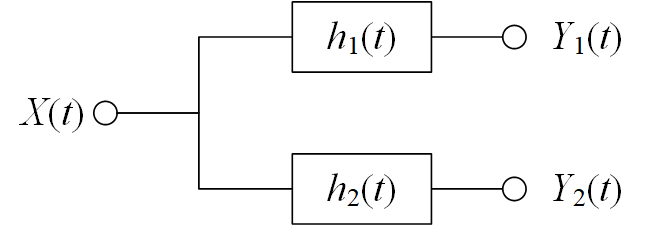
\includegraphics[width=0.8\textwidth]{信号发生器示意图.png}
  \caption{信号滤波器}
  \label{fig:信号滤波器}
\end{figure}

\subsection{设计思路}
首先从原理上讨论应该如何设计两个线性系统,考虑两个输出信号之间的互相关函数。即有:
\begin{equation}
  \begin{aligned}
    R_{XY}(t_1,t_2) & =E\{y_1(t_1)y_2(t_2)\}                                                                                               \\
                    & =E\{[x_1(t)*h_1(t)][x_2(t)*h_2(t)]\}                                                                                 \\
                    & =E\Big\{\int_{-\infty}^{+\infty}x_1(u)h_1(t_1-u)\mathrm{d}u\int_{-\infty}^{+\infty}x_2(v)h_2(t_2-v)\mathrm{d}v\Big\} \\
                    & =\int_{-\infty}^{+\infty}\int_{-\infty}^{+\infty}h_1(t_1-u)h_2(t_2-v)E[x_1(u)x_2(v)]\mathrm{d}u\mathrm{d}v           \\
                    & =\int_{-\infty}^{+\infty}\int_{-\infty}^{+\infty}R_x(u,v)h_1(t_1-u)h_2(t_2-v)\mathrm{d}u\mathrm{d}v                  \\
                    & =R_x(t_1,t_2)*h_1(t_1)*h_2(t_2)
  \end{aligned}
\end{equation}
可见,两个输出信号之间的互相关函数相当于对输入信号的自相关函数进行两次卷积,如果输入的函数是平稳的,两个输出的信号之间是联合平稳的,则可以使用功率谱密度函数表示上述结果,得到以下形式:
\begin{equation}
  \begin{aligned}
    S_{XY}(\omega) & =S_X(\omega)H_1(\omega)H_2^*(\omega)
  \end{aligned}
\end{equation}
可见,当两个输出信号之间的互相关函数为零时,功率谱密度函数也为0,则需要两个线性系统的频率响应函数在每一个频率上均是乘积为0的。换言之,需要设计两个线性系统,使得两个系统的频率响应函数不为零的位置相互错开,即可得到两个输出不相关的信号。

考虑最简单的情况,即设计一个低通滤波器和一个高通滤波器,使得两个滤波器的截止频率相互错开,其在频率上的乘积即可以满足近似为0。工程上,认为阻带内的衰减小于-15dB即可认为是0,滤波器的截止频率定义为幅频增益为-3dB处的频率。\cite*{signal_system}。
\subsection{设计过程}
由于问题没有给任何信号的具体形式,这里也没有必要定义某一个具体的截止频率,不妨设低通滤波器的截止频率(角频率)是$\omega_1$,高通滤波器的截止频率是$\omega_2$,则有:
\subsubsection{低通滤波器}
如下图,低通滤波器的幅频特性为:
\begin{figure}[H]
  \centering
  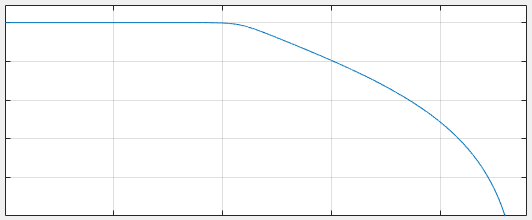
\includegraphics[width=0.8\textwidth]{低通滤波器.png}
  \caption{低通滤波器幅频特性说明}
  \label{fig:低通滤波器}
\end{figure}

可将低通滤波器的频率特性写为:
\begin{displaymath}
  H_1(j\omega)=\frac{1}{\displaystyle 1+j\frac{\omega}{\omega_L}}
\end{displaymath}
其中$\omega_L$为截止频率。
\subsection{高通滤波器}
同理,对于高通滤波器,其幅频特性为:
\begin{figure}[H]
  \centering
  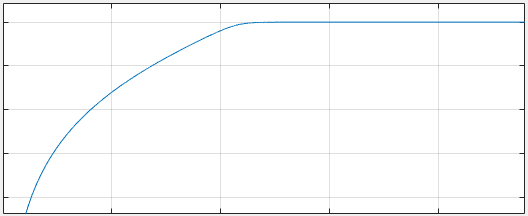
\includegraphics[width=0.8\textwidth]{高通滤波器.png}
  \caption{高通滤波器幅频特性说明}
  \label{fig:高通滤波器}
\end{figure}
可将高通滤波器的频率特性写为:
\begin{displaymath}
  H_2(j\omega)=\frac{1}{\displaystyle 1+j\frac{\omega_H}{\omega}}
\end{displaymath}
其中$\omega_H$为高通截止频率。
\subsubsection{设计结果}
需要注意的是,首先应当保证高通滤波器的截止频率高于低通滤波器的截止频率,即有:
\begin{equation*}
  \omega_2>\omega_1
\end{equation*}

其次是为了保证在任意频率处的幅值增益都小于-15dB,则需要在两个幅频特性相等的位置处,幅值增益的和也小于-15dB,即有:
\begin{align}
  \left\{
  \begin{aligned}
     & 20\lg\mmode{\frac{1}{\displaystyle 1+j\frac{\omega}{\omega_L}}}=20\lg\mmode{\frac{1}{\displaystyle 1+j\frac{\omega_H}{\omega}}}     \\\\
     & 20\lg\mmode{\frac{1}{\displaystyle 1+j\frac{\omega}{\omega_L}}}+20\lg\mmode{\frac{1}{\displaystyle 1+j\frac{\omega_H}{\omega}}}<-15
  \end{aligned}
  \right.
\end{align}
对于某一个给定的截止频率,可得两幅频特性曲线之交点频率,以及两个截止频率需要满足的条件为:
\begin{align*}
  \left\{
  \begin{aligned}
     & \omega=\sqrt{\omega_H\omega_L}                       \\\\
     & \frac{\omega_L^2}{\omega_H^2+\omega_L^2}<10^{-0.375}
  \end{aligned}
  \right.
\end{align*}
因此可以设计得到在任意频率点处,均可以以-15dB负增益。则从输入到输出的功率谱密度函数为:
\begin{align*}
  S_{XY}(\omega)=\frac{S_X(\omega)}{\displaystyle 1+\frac{\omega_H}{\omega_L}+j\circbrac{-\frac{\omega_H}{\omega}+\frac{\omega}{\omega_L}}}
\end{align*}
其中,一个比较简单的实现形式为:
\begin{align*}
  H_1(j\omega)=\frac{1}{\displaystyle 1+j\frac{\omega}{\omega_L}} \implies h_1(t)=\left\{
  \begin{aligned}
     & e^{\displaystyle -\frac{1}{\omega_L}t} & ,  t>0   \\
     & 0                                      & ,  t\le0
  \end{aligned}
  \right.
\end{align*}

\begin{align*}
  H_2(j\omega)=\frac{1}{\displaystyle 1+j\frac{\omega_H}{\omega}} \implies h_1(t)=\left\{
  \begin{aligned}
     & 0                                               & , t>0   \\
     & \delta(t)-e^{\displaystyle \frac{1}{\omega_H}t} & , t\le0
  \end{aligned}
  \right.
\end{align*}\par
这里的高通滤波器是物理不可实现的,因此常常使用巴特沃斯滤波器或者切比雪夫滤波器形式的函数实现高通滤波,而不是使用指数函数的形式,给定截止频率和阻带衰减,即可以设计出对应的高通滤波器。
\section{第二次大作业}
\subsection{概述}
%分析一个应用泊松随机过程的实例。
本文将主要讨论一种新型的神经网络模型,即脉冲神经网络(Spiking Neural Networks,SNN)。该网络据传是继感知机、卷积神经网络之后所谓的第三代类脑仿生网络模型,与前两代神经网络相比,脉冲神经网络在能耗上和存储占用上有着更加突出的优点。但是,当前脉冲神经网络的研究还很不充分,尚未形成一种通用的数学模型基础,因此其模型底层原理、模型训练方法以及模型的推理方法均未见到有通行的方法,大多数研究尚局限在某一具体方法中的应用。从大脑工作机理的仿生学中抽象数学模型、完成对神经元和网络连接拓扑的建模,是当前脉冲神经网络原理领域需要深入研究的工作。本文将针对这一问题,利用随机过程数学工具,对脉冲神经元进行建模,以期望能够归纳出一种通行的模型范式。
\subsection{必要的数学知识}
SNN的输入与输出均是脉冲型信号,根据文献\cite{jaegerEncyclopediaComputationalNeuroscience2015},描述脉冲信号通常使用脉冲序列。
\subsubsection{符号说明}
\begin{enumerate}
  \item 脉冲\textbf{电流信号}使用增量序列表示,记为$X(t)$,常用冲激函数串表示:$X(t)=\sum_i\delta(t-t_i)$,其中$t_i$是产生事件的时刻;
  \item 神经元的输入电流记为$X_i(t)$,输出电流记为$Y(t)$,输入过程是泊松分布过程;
  \item 神经元膜内外电位差用符号$V(t)$表示,简称为“膜电位”;
  \item 神经元放电的阈值膜电位记为$V_T$,膜电位的零位记为$V_0$;
  \item 神经元膜电位时间常数为$\tau$,膜电阻记为$r$;
\end{enumerate}
\subsubsection{泊松过程时间量}
根据\cite{ZhouYinQingSuiJiGuoChengLiLun2013},泊松过程的各事件到达时间$T_i$和相邻两个事件到达时间间隔$Z_i=T_{i+1}-T_i$是两个重要的衍生随机过程,其中到达时间的分布可按泊松过程等价事件概率之和求出,如下式:
\begin{align}
  F_{T_i}(t)=\left\{
  \begin{aligned}
     & 1-\sum\limits_{k=1}^{i-1}e^{-\lambda t}\frac{(\lambda t)^k}{k!} & , t>0    \\
     & 0                                                               & , t\le 0
  \end{aligned}
  \right.
  \label{eq:到达时间概率分布函数}
\end{align}\par
对上式求导可得到其概率分布密度函数,称该分布函数为服从参数$\lambda,i-1$的伽马分布,如下式:
\begin{align}
  f_{T_i}(t)=\left\{
  \begin{aligned}
     & \lambda e^{-\lambda t}\frac{(\lambda t)^{i-1}}{(i-1)!} & ,t>0     \\
     & 0                                                      & , t\le 0
  \end{aligned}
  \right.
  \label{eq:到达时间概率密度函数}
\end{align}\par
类似地,到达时间间隔的分布也可按等价事件求出,其服从强度为$\lambda$的指数分布,即:
\begin{align}
  f_{Z_i}(t)=\left\{
  \begin{aligned}
     & \lambda e^{-\lambda t} & ,t>0    \\
     & 0                      & ,t\le 0
  \end{aligned}
  \right.
  \label{eq:到达时间间隔概率密度函数}
\end{align}\par
后文中将使用到以上两种衍生的随机过程。
\subsubsection{泊松脉冲序列}
本文将主要讨论输入为泊松脉冲序列的情况,因此首先介绍泊松脉冲序列的定义。泊松脉冲序列是一种随机过程,其定义为泊松随机过程的微分过程\cite{ZhouYinQingSuiJiGuoChengLiLun2013},设$N(t)$泊松过程,则泊松脉冲序列定义为:
\begin{align}
  X(t)=\diff{N(t)}{t}=\sum\limits_{i=1}^{+\infty}\delta(t-t_i)
  \label{eq:泊松脉冲序列定义}
\end{align}\par
若设泊松过程$N(t)$的强度为$\lambda$,则泊松脉冲序列的均值为$\lambda$。泊松脉冲序列的自相关函数按均方微分的定义,即:
\begin{align}
  R_X(t_1,t_2)=E\rectbrac{\lim_{\Delta t\to 0}\frac{N(t_1+\Delta t)-N(t_1)}{\Delta t}\frac{N(t_2+\Delta t)-N(t_2)}{\Delta t}}=\lambda^2+\lambda\delta(t_1-t_2)
  \label{eq:泊松脉冲序列自相关函数}
\end{align}\par
求解过程中使用到了脉冲函数的初等函数定义,即脉冲函数等于三角形脉冲在持续时长趋于0的极限。

\subsection{脉冲神经元模型}
脉冲神经元是对神经元细胞生物机理的仿生抽象。目前较为流行的脉冲神经元模型有漏积分放电、脉冲响应、活动频率模型,本文将主要讨论一种较为直观的模型——漏积分放电模型,并尝试将基于该模型得到的结论推广至其他模型。
\subsubsection{数学模型介绍}
根据神经细胞领域的研究\cite{albesa-gonzalezLearningFilopodiaSpines2023},神经元仅当其动作电位(Active Potential)高于其活动阈值后,神经元细胞膜表面的离子通道(通常是钾、钙离子通道)在膜内外电位差的驱动下打开,神经元膜内的钾离子和钙离子将在极短的时间内从膜内释放至膜外,宏观上形成了一次放电时间极短的输出电流,在数学上通常建模为一次总放电能量有限但功率无限的信号,即冲激信号。\par
神经元彼此间通过突触连接,突触是一种化学物质受体,用于接受前一个神经元释放的神经介质。例如,当前一个神经元兴奋时(即产生正电流输出),其释放的神经介质通常为谷氨酸(Glutamate),谷氨酸将与突触上的受体结合,使得后一个神经元膜上的抽运离子通道打开,后一个神经元膜内钠离子浓度提高,导致其膜电位升高。而当前一个神经元抑制时(即产生负电流输出),其释放的神经介质通常为$\gamma$-氨基丁酸(GABA),GABA将与突触上的受体结合,导致后一个神经元抽运阴离子至胞内(常为氯离子),使其膜电位下降。根据离子扩散现象,胞内的高浓度离子也将自发地穿过细胞膜扩散至膜外直到膜两则浓度相同,当神经元长期处于静息状态时,其离子扩散速率等于神经元的抽运速率,膜电位基本稳定在某一固定值。\par
常用的模型是漏积分放电(Leaky Integrate-and-Fire,LIF)神经元\cite{gerstnerTimeStructureActivity1995},即神经元将全部输入脉冲进行线性叠加,微分方程为:
\begin{align}
  \tau\diff{V(t)}{t}=-V(t)+r\sum\limits_iw_iX_i(t)
  \label{eq:LIF积分过程}
\end{align}\par
式中,$X_i(t)$是第$i$个输入脉冲电流,如神经元有多个输入,则将其按权重$w_i$线性叠加;$-V(t)$描述了离子扩散速率,当膜电位较大时,扩散速度较大,因此符合前述一般性假设。神经元的行为不止有积分过程,当膜电位超过膜电位阈值时,神经元放电过程将被激活(Fire),放电过程不是线性过程,可用分段函数表示为:
\begin{align}
  Y(t)=\left\{\begin{aligned}
                1 & ,V(t)>V_T    \\
                0 & ,V(t)\le V_T
              \end{aligned}\right.\implies Y(t)=u\rectbrac{V(t)-V_T}
  \label{eq:LIF放电过程}
\end{align}\par
同时将膜电位置回零位$V_0$,复位过程时间极短,可认为是瞬间完成复位,可用以下方程表示:
\begin{align}
  V(t)=\left\{\begin{aligned}
                V(t) & ,Y(t)=0  \\
                V_0  & ,Y(t)= 1
              \end{aligned}\right.
  \label{eq:LIF复位过程}
\end{align}\par
以上过程可用如下示意图表示,其中下侧方框表示输入脉冲序列,上侧表示输出脉冲序列,中间为神经元膜电位,横坐标是时间。由图可知,当神经元静息时,其膜电位等于静息电位$V_0$,当神经元接受输入脉冲序列后,膜电位$V(t)$迅速上升,在较短时间内达到峰值,然后缓慢下降(Leak),如果前后两次输入脉冲到达时间较长,则由于漏电效应不能产生神经冲动;只有当相邻两次输入脉冲到达时间足够短时,神经元膜电位在短时间内达到阈值电位,从而产生神经冲动(Fire)。图中没有画出多个输入突触的情况。
\begin{figure}[H]
  \centering
  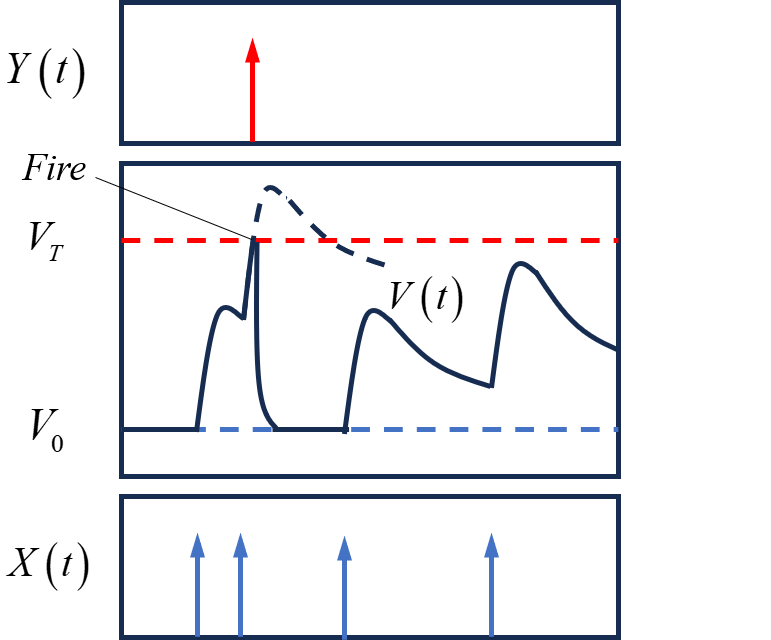
\includegraphics[width=0.8\textwidth]{神经冲动示意图.png}
  \label{fig:神经冲动示意图}
  \caption{单输入作用下的神经冲动示意图}
\end{figure}
至此,基于LIF和脉冲序列的基本神经元模型已经介绍完毕。

\subsection{LIF神经元学习过程}
与感知机相同,LIF神经元也能够从大量的输入抽取内含的信息,完成无监督学习,从而实现对输入的分类。输入的脉冲增量序列可以看作是独立增量过程,神经元充当分类器,将输入的脉冲序列完成分类。考虑一种较为简单的情况,即将输入的脉冲序列看作是泊松脉冲列\cite{ZhouYinQingSuiJiGuoChengLiLun2013,NIPS2009_a5cdd4aa},分类器根据脉冲列强度的数值分类。\par
\subsubsection{膜电位增量}
分类器由数据驱动,这里可供学习的隐含参数有三个,一个是脉冲神经元的膜电位时间常数$\tau$,一个是脉冲神经元突触的权重$w_i$以及脉冲神经元活动阈值电位$V_T$。实际上,阈值电位与神经元膜离子通道的组成和数量有关,通常同一类神经元其阈值电位都是相同的,(可类比感知神经元中的激活函数都是同一个函数,如Relu函数),也为了简化分析,不妨设神经元活动阈值电位是某个固定值(如常取为0)。另外两个参数可供学习改变,仅考虑一个神经元在单次输入下的学习过程,合并膜电阻$r$和突触权重$w$,将方程\ref{eq:LIF积分过程}简化为:
\begin{align}
  \tau\diff{V(t)}{t}=-V(t)+rwX(t)=-V(t)+\tilde{w}X(t)
  \label{eq:LIF简化积分过程}
\end{align}\par
忽略放电过程,直接在初值条件下联立\ref{eq:泊松脉冲序列定义}和\ref{eq:LIF简化积分过程},得到:
\begin{align}
  V(t)=\frac{\tilde{w}}{\tau}\sum\limits_{i}u(t-t_i)e^{-\frac{t-t_i}{\tau}}+\frac{V_0}{\tau}e^{-\frac{t}{\tau}}
  \label{eq:LIF膜电位公式}
\end{align}\par
可见该式较为复杂,膜电位仍然是随机过程,但是不能从表达式上推断其性质。忽略求和号前面的常数项,初始值的指数衰减不受脉冲输入的影响,因此可以仅考虑膜电位的增量过程$\Delta V_i(t)$,可知:
\begin{align}
  \Delta V_i(t)=u(t-t_i)e^{-\frac{t-t_i}{\tau}}
  \label{eq:不考虑放电的膜电位增量}
\end{align}\par
利用公式\ref{eq:不考虑放电的膜电位增量},在不考虑放电的条件下,可计算膜电位增量的概率分布。根据全概率公式,有:
\begin{align}
  \begin{aligned}
    P\curlbrac{\Delta V_i(t)\le v} & =P\curlbrac{\Delta V_i(t)\le v|t\le t_i}P\curlbrac{t\le t_i}+P\curlbrac{\Delta V_i(t)\le v|t> t_i}P\curlbrac{t>t_i}                                                    \\
                                   & =1\cdot\sum_{k=0}^{i-1}e^{-\lambda t}\frac{(\lambda t)^k}{k!}+P\curlbrac{\Delta V_i(t)\le v|t> t_i}\rectbrac{1-\sum_{k=0}^{i-1}e^{-\lambda t}\frac{(\lambda t)^k}{k!}}
  \end{aligned}\label{eq:膜电位增量概率分布}
\end{align}\par
注意到零位电位为0,膜电位放电不会产生负电位,因此$v<0$的情况以概率0发生;同时,增量过程所能取得的最大值为1,因此$v>1$的情况以概率1发生。对于条件概率$P\curlbrac{\Delta V_i(t)\le v|t> t_i}$,由于时间为脉冲$t_i$之后,此时增量不为0,因此可利用等价事件原理,结合公式\ref{eq:到达时间概率密度函数}和贝叶斯公式,将上述概率改写为:
\begin{align}
  \begin{aligned}
    P\curlbrac{\Delta V_i(t)\le v|t> t_i} & =P\curlbrac{ue^{-\frac{t-t_i}{\tau}}\le v\Big|t> t_i}                                                                                                                     \\
                                          & = P\curlbrac{t_i\le t+\tau\ln\frac{v}{u}\Big|t> t_i}                                                                                                                      \\
                                          & =P\curlbrac{t_i\le t(v)|t> t_i}                                                                                                                                           \\
                                          & =\left\{\begin{aligned}
                                                       & 1                                                                                                                                     & ,v>1                   \\
                                                       & \displaystyle\frac{1-\sum_{k=0}^{i-1}e^{-\lambda t(v)}{[\lambda t(v)]^k}/{k!}}{1-\sum_{k=0}^{i-1}e^{-\lambda t}{(\lambda t)^k}/{k!} }
                                                       & ,e^{-\frac{t}{\tau}}\le v\le 1                                                                                                                                 \\
                                                       & 0                                                                                                                                     & ,v<e^{-\frac{t}{\tau}}
                                                    \end{aligned} \right.
  \end{aligned}\label{eq:求膜电位增量的等价事件}
\end{align}\par
说明:式中的$\displaystyle t(v)=t+\tau\ln\frac{v}{u}$,其中$u=1\unit{A}$是量纲为电流的常数。联立公式\ref{eq:膜电位增量概率分布}和公式\ref{eq:求膜电位增量的等价事件},可解出膜电位增量的概率密度分布函数:
\begin{align}
  \begin{aligned}
    F_{\Delta V_i}(v,t) & =P\curlbrac{\Delta V_i(t)\le v}                                                                                                                                                                       \\
                         & =1\cdot\left\{
                          \begin{aligned}
                            & \sum_{k=0}^{i-1}e^{-\lambda t}\frac{(\lambda t)^k}{k!} & ,v\ge 0         \\
                                                                                    & 0       & ,v< 0
                           \end{aligned}\right.+\left\{\begin{aligned}
                                                          & 1-\sum_{k=0}^{i-1}e^{-\lambda t}\frac{(\lambda t)^k}{k!},      & v>1                    \\
                                                          & 1-\sum_{k=0}^{i-1}e^{-\lambda t(v)}\frac{[\lambda t(v)]^k}{k!}
                                                          & ,e^{-\frac{t}{\tau}}\le v\le 1                                                          \\
                                                          & 0                                                              & ,v<e^{-\frac{t}{\tau}}
                                                       \end{aligned} \right.                                                        \\
                         & =\left\{\begin{aligned}
                                      & 1                                                                                                                     & ,v>1                              \\
                                      & 1-\sum_{k=0}^{i-1}e^{-\lambda t(v)}\frac{[\lambda t(v)]^k}{k!}+\sum_{k=0}^{i-1}e^{-\lambda t}\frac{(\lambda t)^k}{k!} & , e^{-\frac{t}{\tau}} \le v \le 1 \\
                                      & \sum_{k=0}^{i-1}e^{-\lambda t}\frac{(\lambda t)^k}{k!}                                                                & ,0\le v<e^{-\frac{t}{\tau}}       \\
                                      & 0                                                                                                                     & ,v<0
                                   \end{aligned}\right.
  \end{aligned}
\end{align}\par
而对于增量过程而言,一次只能出现一个增量,不能同时产生两个,因此$i=1$,上式可以化简为:
\begin{align}
  F_{\Delta V}(v,t) =\left\{\begin{aligned}
                                & 1                                                                     & ,v>1                              \\
                                & \displaystyle 1-\frac{e^{-\lambda t}}{v^{\lambda\tau}}+e^{-\lambda t} & , e^{-\frac{t}{\tau}} \le v \le 1 \\
                                & e^{-\lambda t}                                                        & ,0\le v<e^{-\frac{t}{\tau}}\\
                                & 0                                                                     & ,v<0
                             \end{aligned}\right.\label{eq:膜电位增量的分布}
\end{align}\par
对变量$v$求导,可得到膜电位增量分布的概率密度函数,注意此时\textbf{没有考虑放电}:
\begin{align}
  f_{\Delta V_i}(v,t)=\left\{
  \begin{aligned}
     & \displaystyle\frac{\lambda\tau}{v}e^{-\lambda t(v)}\frac{[\lambda t(v)]^{i-1}}{(i-1)!} & ,e^{-\frac{t}{\tau}} \le v \le 1 \\
     & 0                                                                                      & ,\textrm{其他}
  \end{aligned}
  \right.
\end{align}\par
同理,取$i=1$,得到:
\begin{align}
  f_{\Delta V}(v,t)=\left\{
  \begin{aligned}
     & \frac{\lambda\tau}{v^{\lambda \tau+1}}e^{-\lambda t} & ,e^{-\frac{t}{\tau}} \le v \le 1 \\
     & 0                                                    & ,\textrm{其他}
  \end{aligned}
  \right.\label{eq:膜电位增量的概率密度函数}
\end{align}\par
\subsubsection{膜电位量}
脉冲神经元的膜电位决定了其输出脉冲序列的一切分布特性,因此首先分析的是膜电位量,不考虑放电的影响,设随机过程$V(t)$为脉冲神经元在时刻$t$的膜电位随机量,膜电位初始值置为$V_0$,则可以求得电位的条件概率分布为:
\begin{align}
  \begin{aligned}
    P\curlbrac{V(\Delta t)\le v
    \big|  N(\Delta t)=n}  =P\curlbrac{\frac{\tilde{w}}{\tau}\sum_{i=1}^{n}\Delta V_i(\Delta t)+\frac{V_0}{\tau}e^{-\frac{\Delta t}{\tau}}\le v\Big| N(\Delta t)=n,0<\Delta t\le t_2-t_1}            \\
                    =P\curlbrac{\sum_{i=1}^{n}\Delta V_i(\Delta t)\le \frac{\tau}{\tilde{w}}\circbrac{v-\frac{V_0}{\tau}e^{-\frac{\Delta t}{\tau}}}\Big| N(\Delta t)=n,0<\Delta t\le t_2-t_1}
  \end{aligned} \label{eq:膜电位的条件分布概率}
\end{align}\par
式中的随机过程$N(t)$表示从初始时刻到时刻$t$的时间段内,输入脉冲序列的脉冲个数,显然该随机过程是一个泊松过程。根据公式\ref{eq:LIF膜电位公式}可知,该随机过程是由输入随机序列$X(t)$与指数衰减过程的复合随机过程,输入随机序列服从泊松分布,因此可将膜电位量写成如下的复合随机过程形式:
\begin{align}
  V(t)=\sum_{k=1}^{N(t)}e^{-\frac{t-t_k}{\tau}}
  \label{eq:膜电位量复合随机过程形式}
\end{align}\par
式中,$t_k,k=1,2,\cdots,N(t)$表示第$k$个输入脉冲的到达时间,其中$0\le t_1\le t_2\le\cdots\le t_{N(t)}<t$均落在时间段$[0,t)$范围内。根据复合泊松随机过程的期望和方差,可求得膜电位量$V(t)$在公式\ref{eq:膜电位量复合随机过程形式}表达下的期望,即有:
\begin{align}
  \begin{aligned}
  \expec{V(t)}&=\expec{\expec{\sum_{k=1}^{n}e^{-\frac{t-t_k}{\tau}}\Big|N(t)=n}}\\
  &=\expec{N(t)}\expec{e^{-\frac{t-t_k}{\tau}}}\\
  &=\int_{0}^{t}t_k\frac{1}{t_k}e^{-\frac{t-t_k}{\tau}}\di t_k\cdot \lambda t\\
  &=\lambda t\cdot\frac{1-e^{- t/\tau}}{ t/\tau}=\lambda\tau\circbrac{1-e^{- t/\tau}}
\end{aligned} \label{eq:膜电位量的期望}
\end{align}\par
说明:式中对$t_k$求期望时,由于到达时间在条件$N(t)=n$下的分布服从均匀分布,因此该式可直接使用均匀分布求取。
\subsection{放电过程}
放电过程中涉及到非线性系统,放电过程仅有两种取值可能,即放电或不放电。设某两次放电的时刻为$t_1$和$t_2$,则在$t_1$和$t_2$时刻内,神经元不产生放电现象,在该时间段内,膜电位的条件分布概率如公式\ref{eq:膜电位的条件分布概率}所示,根据全概率公式,可算出在该时间段内的膜电位分布:
\begin{align}
  \begin{aligned}
    F_{V(t)|t_1\le t\le t_2}(v)=    \sum_{n=1}^{\infty}P\curlbrac{\sum_{i=1}^{n}\Delta V_i(t)\le \frac{\tau}{\tilde{w}}\circbrac{v-\frac{V_0}{\tau}e^{-\frac{t}{\tau}}}\Big| N(t_2)-N(t_1)=n,t_1\le t\le t_2}\cdot \\
    P\curlbrac{ N(t_2)-N(t_1)=n,t_1\le t\le t_2}
  \end{aligned}
\end{align}\par
在$t_1$到$t_2$时刻内未产生放电现象,设$T_i(t)$表示第i个输出信号的到达时间,有以下式成立:
\begin{align*}
   & P\curlbrac{T_2-T_{1}>t_2-t_1}=P\curlbrac{Y(t)=0|t_1\le t\le t_2}                                                      \\
   & =  P\curlbrac{V(t)\le V_T|t_1\le t\le t_2}                                                                \\
   & = P\curlbrac{\frac{V_0}{\tau}e^{-\frac{t}{\tau}}+V(t_1+\Delta t)-V(t_1)\le V_T\Big|0<\Delta t\le t_2-t_1}
\end{align*}\par
根据全概率公式,对时间段内产生的脉冲数事件求全集,得到以下结果:
\begin{align}
  \begin{aligned}
     & P\curlbrac{\frac{V_0}{\tau}e^{-\frac{t}{\tau}}+V(t_1+\Delta t)-V(t_1)\le V_T\Big|0<\Delta t\le t_2-t_1} \\
     &=\sum_{n=1}^{\infty}P\curlbrac{\sum_{i=1}^{n}\Delta V_i(\Delta t)\le \frac{\tau}{\tilde{w}}\circbrac{V_T-\frac{V_0}{\tau}e^{-\frac{\Delta t}{\tau}}}\Big| N(t_2)-N(t_1)=n,0<\Delta t\le t_2-t_1}\\
     & \quad\cdot  P\curlbrac{ N(t_2)-N(t_1)=n,0<\Delta t\le t_2-t_1}                                                 
  \end{aligned}
  \label{eq:放电过程等价事件全集}
\end{align}\par
取$\displaystyle \tilde{V}_T= \frac{\tau}{\tilde{w}}\circbrac{V_T-\frac{V_0}{\tau}e^{-\frac{\Delta t}{\tau}}}$。
在使用脉冲神经元时,需要根据数据更新神经元参数,主要是权重值$w$,这里对比输出、输入脉冲序列的强度来更新权重参数。求解输出脉冲序列的强度需要使用输出脉冲到达时间间隔的期望,结合公式\ref{eq:LIF放电过程},可将放电过程用膜电位量改写为:
\begin{align}
  Y(t)=u\rectbrac{\sum_{k=1}^{N(t)}e^{-\frac{t-t_k}{\tau}}-V_T}
  \label{eq:输出脉冲随机过程的定义}
\end{align}\par
可见放电过程是非线性过程,前后两次输出脉冲序列可根据等价事件写为:
\begin{align*}
   \prob{Y(t_1)=1,Y(t_2)=1,V(t)<\tilde{V}_T}=\prob{V(t_1)\ge \tilde{V}_T,V(t_2)\ge \tilde{V}_T,V(t)<\tilde{V}_T},t_1\le t\le t_2
\end{align*}\par
求解前后两次输出脉冲的时间间隔,再次使用等价事件,写为:
\begin{align*}
  \prob{\Delta S=S_2-S_1>s}&=\prob{V(s_1)< \tilde{V}_T , V(s_1+s)< \tilde{V}_T,V(t)<\tilde{V}_T}\\
  \prob{\Delta S=S_2-S_1\le s}&=s_2-s_1-\prob{V(s_1)< \tilde{V}_T , V(s_1+s)< \tilde{V}_T,V(t)<\tilde{V}_T},s_1\le t\le s_2
\end{align*}\par
进一步求解输出时间间隔的期望,得到以下形式:
\begin{align*}
  \expec{\Delta S}&=\sum_{s}s\prob{\Delta S=S_2-S_1\le s}\\
&=\sum_{s}s\rectbrac{1-\prob{V(s_1)< \tilde{V}_T , V(s_1+s)< \tilde{V}_T,V(t)<\tilde{V}_T}}
\end{align*}\par
可见时间间隔的期望与初始时刻$s_1$有关,输出脉冲过程不是平稳的。在实际使用中,每次完成两次输出脉冲,可将计时器回零。求解时间间隔的分布需要使用膜电压量的分布,而根据公式\ref{eq:输出脉冲随机过程的定义},膜电压量概率分布的直接表达式很难求解(实际上是不解析的)。将\ref{eq:膜电位量的期望}代入上式,间接地求解其放电脉冲序列时间间隔,即有:
\begin{align*}
  \expec{\Delta S}\expec{V(t)}&\approx\int_{0}^{+\infty}s\diff{\prob{V(s_1+s)< \tilde{V}_T,V(t)<\tilde{V}_T}}{s}\di s\expec{\expec{\sum_{k=1}^{n}e^{-\frac{t-t_k}{\tau}}\Big|N(t)=n}}\\
  &=\int_{0}^{+\infty}s\diff{\prob{V(s_1+s)< \tilde{V}_T,V(t)<\tilde{V}_T}}{s}\di s\int_{0}^{t}t_k\frac{1}{t_k}e^{-\frac{t-t_k}{\tau}}\di t_k\cdot \lambda t\\
  &=\int_{0}^{+\infty}\di s\int_{0}^{t} se^{-\frac{t-t_k}{\tau}}\diff{\prob{V(s)< \tilde{V}_T,V(t)<\tilde{V}_T}}{s}\di t_k\cdot \lambda t\\
  &\approx \tilde{V}_T\tau\circbrac{1-e^\frac{t}{\tau}}
\end{align*}\par
式中,使用到了计时器回零操作$s_1=0$。因此有:
\begin{align}
  \expec{\Delta S} =\frac{\tilde{V}_T\tau\circbrac{1-e^{-\frac{t}{\tau}}}}{\expec{V(t)}}\implies \expec{\Delta S}=\frac{\tilde{V}_T}{\lambda}
\end{align}\par
因此联合公式\ref{eq:放电过程等价事件全集},在初始膜电位取0的情况下,可以使用权重和门限电压值表示出近似的输出脉冲时间间隔期望:
\begin{align}
  \expec{\Delta S}=\frac{\tau}{\lambda\tilde{w}}V_T
  \label{eq:近似的输出脉冲时间间隔期望值}
\end{align}\par
\newpage
\printbibliography[heading=bibliography,title=参考文献]
\end{document}
